% Adaptacion de la plantilla replab suministrada: dos columnas,
% secciones romanas y referencias numeradas siguiendo convenciones IEEE.
\documentclass{replab}
\usepackage{listings}
\usepackage{booktabs}
\usepackage{float}
\definecolor{MidnightBlue}{HTML}{003D64}
\setlength{\columnsep}{18pt}
\renewcommand{\thesection}{\Roman{section}}
\renewcommand{\thesubsection}{\Alph{subsection}}
\titleformat{\section}{\centering\normalfont\normalsize\bfseries}{\thesection.}{0.6em}{}
\titleformat{\subsection}{\normalfont\normalsize\itshape}{\thesubsection.}{0.6em}{}
\titlespacing*{\section}{0pt}{10pt}{6pt}
\titlespacing*{\subsection}{0pt}{7pt}{4pt}
\captionsetup{font=footnotesize,labelfont=bf,margin=0pt}
\lstset{language=Verilog,basicstyle=\ttfamily\scriptsize,
 keywordstyle=\bfseries\color{principaluno},commentstyle=\color{gray},
 numbers=left,numberstyle=\tiny\color{gray},numbersep=5pt,
 frame=single,rulecolor=\color{lightgray},breaklines=true,
 showstringspaces=false,tabsize=4,aboveskip=5pt,belowskip=7pt}
\hypersetup{pdftitle={Registros SISO, SIPO, PISO y PIPO en Verilog},pdfauthor={Juan Fernando Zapata Valderrama}}
\author{\textbf{Nombre:} Juan Fernando Zapata Valderrama\\
\href{mailto:fernando.zapata@utp.edu.co}{\texttt{fernando.zapata@utp.edu.co}}}
\makeatletter
\newcommand{\autorinforme}{\@author}
\makeatother
\pagestyle{fancy}
\fancyhf{}
\fancyhead[L]{\footnotesize Electrónica Digital}
\fancyhead[R]{\footnotesize Registros de cuatro bits}
\fancyfoot[C]{\footnotesize\thepage}
\renewcommand{\headrulewidth}{0.3pt}
\begin{document}
\selectlanguage{spanish}
\twocolumn[{
\begin{center}
\begin{minipage}{0.12\textwidth}
\includegraphics[width=\linewidth]{imagenes/escudo-utp.png}\end{minipage}\hfill
\begin{minipage}{0.72\textwidth}\centering
{\Large\bfseries Registros SISO, SIPO, PISO y PIPO\\en Verilog\par}\medskip
{\normalsize \autorinforme\par}\smallskip
{\small Universidad Tecnológica de Pereira\\Electrónica Digital\\19 de noviembre de 2026\par}
\end{minipage}\hfill
\begin{minipage}{0.10\textwidth}
\includegraphics[width=\linewidth]{imagenes/logo-isc.png}\end{minipage}
\end{center}
\vspace{3pt}\hrule\vspace{9pt}
\begin{minipage}{\textwidth}\small
\textbf{Resumen---}Se implementan cuatro registros síncronos de cuatro bits en Verilog: entrada serie y salida serie (SISO), entrada serie y salida paralela (SIPO), entrada paralela y salida serie (PISO), y entrada paralela y salida paralela (PIPO). Se describen sus ecuaciones de transición, el reinicio síncrono y el orden de transmisión. Los circuitos se ejecutaron en DigitalJS; sus capturas relacionan el código con los multiplexores y elementos de memoria. Una verificación adicional en Icarus Verilog compara las salidas con un modelo de referencia durante 6304 ciclos sin discrepancias. La validación corresponde a simulación funcional.\par\smallskip
\textbf{Palabras clave---}Registro, desplazamiento, Verilog, flip-flop D, simulación.\par\smallskip
\textbf{Abstract---}Four synchronous four-bit registers are implemented in Verilog: SISO, SIPO, PISO and PIPO. Their state transitions, synchronous reset and bit order are described. The circuits were run in DigitalJS, whose screenshots are related to the HDL descriptions. An additional Icarus Verilog testbench compares the outputs against a reference model over 6304 cycles with no mismatches. Validation is limited to functional simulation.\par
\end{minipage}\vspace{12pt}
}]

\section{Introducción y objetivo}
Los registros almacenan palabras binarias mediante elementos de memoria controlados por un reloj. La selección de entradas y salidas serie o paralelas permite adaptar la transferencia de información a diferentes interfaces. Como ejemplo comercial de conversión serie a paralelo, el SN74HC595 integra un registro de desplazamiento y otro de almacenamiento de ocho bits \cite{ti}; aquí se estudian versiones didácticas de cuatro bits y un solo reloj.

El objetivo es implementar las cuatro configuraciones, interpretar sus circuitos y comprobar el comportamiento definido por el código. PIPO es un registro de carga paralela; su implementación no realiza desplazamiento interno.

\section{Marco teórico}
\subsection{Memoria y sincronización}
Un flip-flop D captura el valor de su entrada en el flanco activo. Cuatro etapas forman la palabra $Q=(q_3,q_2,q_1,q_0)$. En todos los módulos se utiliza el flanco de subida de \texttt{clk}; \texttt{reset} es síncrono, activo en uno y tiene prioridad. Por tanto, activar reset entre flancos no modifica inmediatamente la salida.

Las asignaciones no bloqueantes \texttt{<=} permiten calcular el siguiente estado usando los valores anteriores. En ausencia de un flanco de subida, el estado se conserva. Antes del primer reinicio, la simulación puede mostrar valores desconocidos, representados por \texttt{x}.

\subsection{Transiciones y orden de los bits}
Sea $Q^+$ el estado posterior al flanco, $s$ la entrada serie, $D$ la palabra paralela, $R$ el reset y $C$ la carga. Para SISO y SIPO:
\begin{equation}
Q^+=\begin{cases}0000,&R=1,\\(q_2,q_1,q_0,s),&R=0.\end{cases}
\end{equation}
SISO expone $q_3$ y SIPO expone $Q$. Un bit capturado en el primer flanco llega a $q_3$ después del cuarto flanco, contando el de captura. Para PISO:
\begin{equation}
Q^+=\begin{cases}0000,&R=1,\\D,&R=0,\ C=1,\\(q_2,q_1,q_0,0),&R=0,\ C=0.\end{cases}
\end{equation}
Su salida es $q_3$: el primer bit está disponible tras el flanco de carga y los siguientes tras cada desplazamiento. En PIPO:
\begin{equation}
Q^+=\begin{cases}0000,&R=1,\\D,&R=0.\end{cases}
\end{equation}

\clearpage
\section{Implementación en Verilog}
Los listados se incluyen directamente desde los archivos entregados. Cada módulo tiene cuatro bits, un reloj y reset síncrono. No existe una señal de habilitación: el registro se actualiza en cada flanco de subida.

\subsection{SISO: entrada serie, salida serie}
El bit nuevo entra por la posición cero. La salida toma la posición tres, mientras las posiciones inferiores se realimentan hacia la siguiente etapa.
\lstinputlisting[firstline=3]{codigo/siso.v}

\subsection{SIPO: entrada serie, salida paralela}
Comparte la transición de SISO, pero permite observar simultáneamente los cuatro bits almacenados. Después de introducir $1,0,1,1$, en ese orden, la palabra es $1011$.
\lstinputlisting[firstline=3]{codigo/sipo.v}

\newpage
\subsection{PISO: entrada paralela, salida serie}
Con \texttt{cargar=1}, la palabra completa reemplaza al estado. Con \texttt{cargar=0}, se desplaza e introduce un cero. Mantener la carga activa vuelve a cargar el dato en cada flanco.
\lstinputlisting[firstline=4]{codigo/piso.v}

\subsection{PIPO: entrada paralela, salida paralela}
Captura simultáneamente las cuatro entradas. Su salida permanece estable entre flancos, aunque cambie la entrada.
\lstinputlisting[firstline=3]{codigo/pipo.v}

\clearpage
% Las figuras abarcan ambas columnas para conservar las etiquetas originales.
\begin{figure*}[p]
\centering
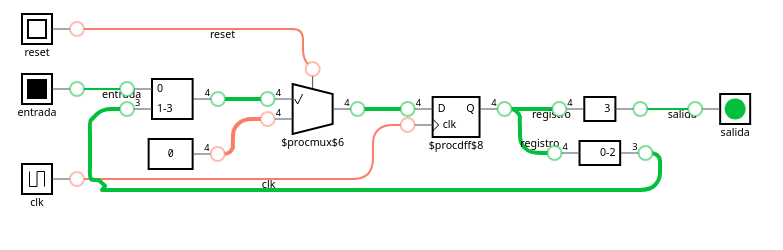
\includegraphics[width=0.83\textwidth]{imagenes/siso.png}
\caption{SISO. El bloque de memoria almacena cuatro bits; la salida selecciona el bit 3 y los bits 2:0 se realimentan al camino de desplazamiento. Captura de DigitalJS aportada por el usuario.}\label{fig:siso}
\vspace{4pt}
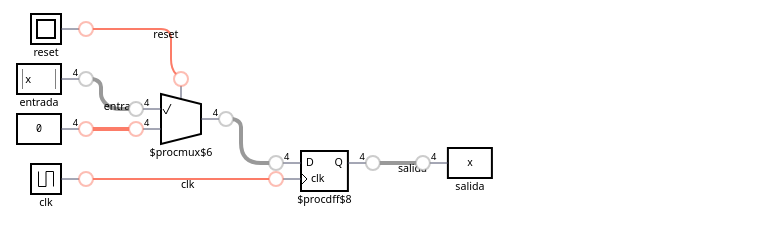
\includegraphics[width=0.83\textwidth]{imagenes/pipo.png}
\caption{PIPO. El multiplexor selecciona la entrada paralela o la palabra cero antes del registro de cuatro bits. La captura muestra valores desconocidos, por lo que no demuestra una carga válida por sí sola.}\label{fig:pipo}
\vspace{4pt}
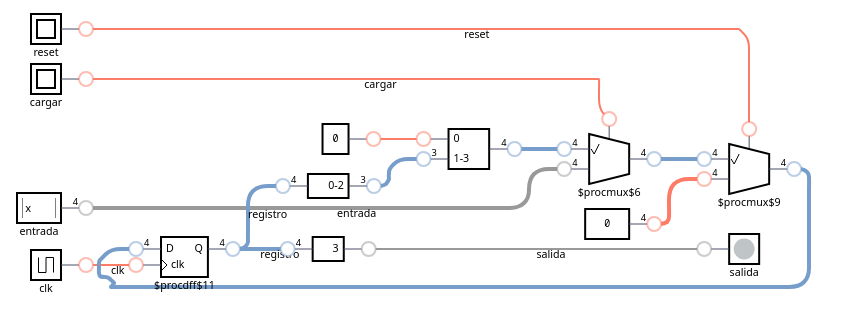
\includegraphics[width=0.83\textwidth]{imagenes/piso.png}
\caption{PISO. Dos multiplexores seleccionan carga o desplazamiento y aplican la prioridad de reset. La selección del bit 3 produce la salida serie.}\label{fig:piso}
\vspace{4pt}
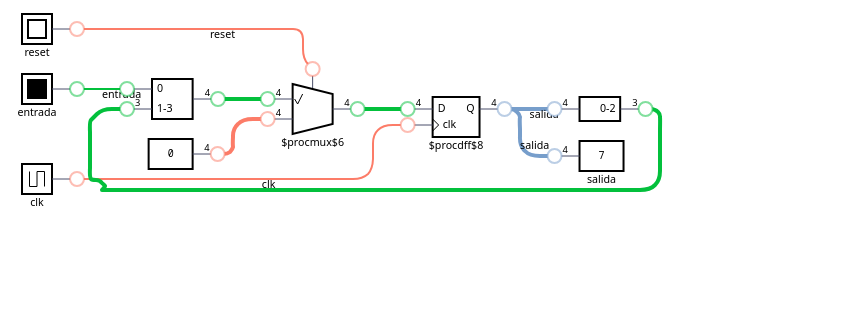
\includegraphics[width=0.83\textwidth,trim=0 95 0 0,clip]{imagenes/sipo.png}
\caption{SIPO. La realimentación de los bits 2:0 implementa el desplazamiento y el bus completo constituye la salida paralela. Se recorta únicamente el margen inferior en blanco para la presentación.}\label{fig:sipo}
\end{figure*}
\clearpage
\small
\section{Análisis de los circuitos}
Los circuitos se ejecutaron en DigitalJS. Las Figuras~\ref{fig:siso}--\ref{fig:sipo} son capturas de ese entorno y corresponden a SISO, PIPO, PISO y SIPO. La identificación se basa en el ancho de las entradas y salidas y en los caminos de realimentación. Un bloque de memoria con bus de cuatro bits representa cuatro elementos de almacenamiento, aunque el dibujo no muestre cuatro símbolos independientes.

En SISO y SIPO, la concatenación combina tres bits del estado anterior con la entrada serie. El multiplexor de reset coloca cero en la entrada de la memoria y el cambio se aplica en el siguiente flanco. En PISO, el multiplexor de carga elige entre la entrada paralela y el desplazamiento; el multiplexor de reset tiene prioridad sobre ambos. PIPO necesita únicamente seleccionar entre el dato paralelo y cero.

Las capturas son instantáneas. Los valores \texttt{x} indican datos desconocidos; por sí solos no identifican su causa.

\section{Verificación y resultados}
\subsection{Procedimiento en Quartus Prime}
Para compilar, se debe crear un proyecto, seleccionar el dispositivo de la placa, agregar el archivo Verilog y establecer su módulo como entidad principal. Después se ejecuta \textit{Analysis \& Synthesis} y se revisa el informe \cite{quartus}. El banco de pruebas no se agrega como hardware sintetizable. Este procedimiento queda pendiente: Quartus no está instalado en el entorno de esta entrega.

\subsection{Pruebas funcionales realizadas}
La organización de estas pruebas se realizó con asistencia de ChatGPT 6.1 Sol. La ejecución visual corresponde a DigitalJS. La comprobación automática de \texttt{registros\_tb.v} se realizó con Icarus Verilog 13.0 y \texttt{vvp} \cite{icarus}. Las entradas cambian en el flanco de bajada y se verifican después del flanco de subida. Estos resultados no se atribuyen a Quartus.

El modelo calcula el desplazamiento mediante multiplicación por dos y módulo 16. Se detectan salidas desconocidas y cambios indebidos entre flancos.

\begin{table}[H]
\centering\small
\caption{Cobertura del banco de pruebas}
\begin{tabular}{p{0.73\columnwidth}r}
\toprule
Grupo & Ciclos\\\midrule
16 patrones: reset, carga, 4 bits y vaciado & 160\\
Transiciones PISO: $16\times2\times2\times16$, con preparación & 2048\\
Secuencia pseudoaleatoria reproducible & 4096\\\midrule
Total comparado con el modelo & 6304\\\bottomrule
\end{tabular}
\end{table}
El grupo PISO recorre todos los estados iniciales, las combinaciones de reset y carga y las 16 palabras de entrada. Cada combinación usa un ciclo de preparación y uno de transición. La secuencia pseudoaleatoria utiliza la semilla hexadecimal \texttt{12345678}.

\subsection{Ejemplo temporal}
Para SISO y SIPO se aplica reset y después la secuencia $1,0,1,1$:
\begin{table}[H]
\centering\small
\caption{Estados tras cada flanco de subida}
\begin{tabular}{cccc}
\toprule
Flanco & Entrada serie & SIPO & SISO\\\midrule
Reset & -- & 0000 & 0\\
1 & 1 & 0001 & 0\\
2 & 0 & 0010 & 0\\
3 & 1 & 0101 & 0\\
4 & 1 & 1011 & 1\\\bottomrule
\end{tabular}
\end{table}
En PISO, cargar $1011$ deja disponible el primer $1$ después de la carga. Los siguientes tres flancos sin carga producen $0$, $1$ y $1$; un cuarto desplazamiento deja el registro en cero. PIPO presenta $1011$ después del flanco que captura esa palabra.

\subsection{Resultado observado y alcance}
Icarus Verilog reportó: \texttt{OK: SISO, SIPO, PISO y PIPO; 6304 ciclos verificados}. No hubo discrepancias con el modelo. El registro está en \texttt{evidencia/simulacion.txt}. No se dispone de un informe de compilación de Quartus ni de pruebas físicas en FPGA. La comprobación cubre las secuencias simuladas; no evalúa frecuencia máxima, tiempos de establecimiento y retención ni consumo.

\section{Conclusiones}
\begin{enumerate}[leftmargin=*,itemsep=3pt]
\item SISO y SIPO comparten la transición interna y difieren en el número de bits expuestos en la salida.
\item PISO transmite primero el bit más significativo, disponible después del flanco de carga.
\item PIPO captura cuatro bits simultáneamente y conserva la salida entre flancos.
\item El reset síncrono requiere un flanco de subida y prevalece sobre la carga, como comprueba la simulación.
\item DigitalJS permitió ejecutar y visualizar los circuitos; los 6304 ciclos de Icarus Verilog aportan una comprobación adicional.
\end{enumerate}

\begingroup\raggedright
\begin{thebibliography}{9}
\bibitem{icarus} Icarus Verilog, \href{https://steveicarus.github.io/iverilog/usage/simulation.html}{``Simulation Using Icarus Verilog''}. Consulta: 19 nov. 2026.
\bibitem{ti} Texas Instruments, \href{https://www.ti.com/product/SN74HC595}{``SN74HC595: 8-bit shift registers''}. Consulta: 19 nov. 2026.
\bibitem{quartus} Intel, \href{https://www.intel.com/programmable/technical-pdfs/683283.pdf}{\textit{Quartus Prime Standard Edition User Guide: Design Compilation}}. Consulta: 19 nov. 2026.
\end{thebibliography}
\endgroup
\end{document}
